\documentclass[11pt,a4paper]{article}

\usepackage{main}
\usepackage{cours}

\renewcommand{\typedocument}{Document}
\renewcommand{\classe}{5e}
\renewcommand{\titre}{Circuits en série et en dérivation}

\begin{document}

\creertitre{Expériences: circuits en série et en dérivation}

On considère un circuit électrique composé d'une lampe et d'un générateur.

\renewcommand{\arraystretch}{1.4}
\begin{tabular}{|>{\bfseries\centering\arraybackslash}m{5cm}|m{7cm}|m{7cm}|}
\hline
\rowcolor{headergrey}
\textbf{Expérience} & \textbf{\centering Circuit en série} & \textbf{\centering Circuit en dérivation} \\
\hline
1. On branche une deuxième lampe 
    & 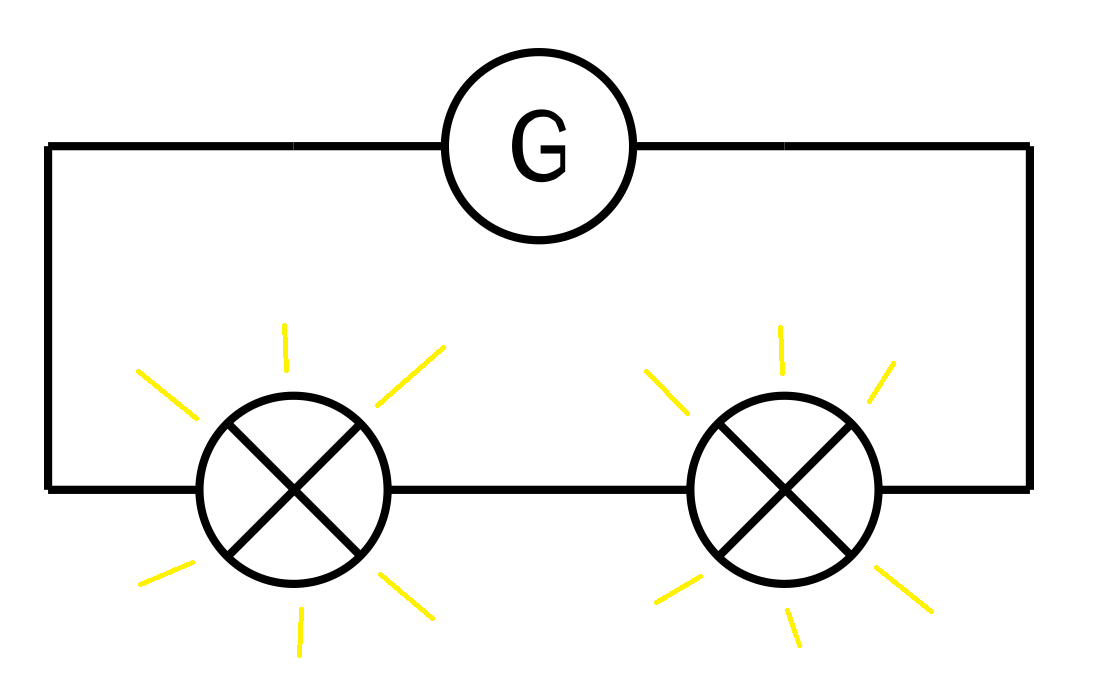
\includegraphics[width=5cm]{images/1s.png}\newline Les lampes brillent moins fort.
    & 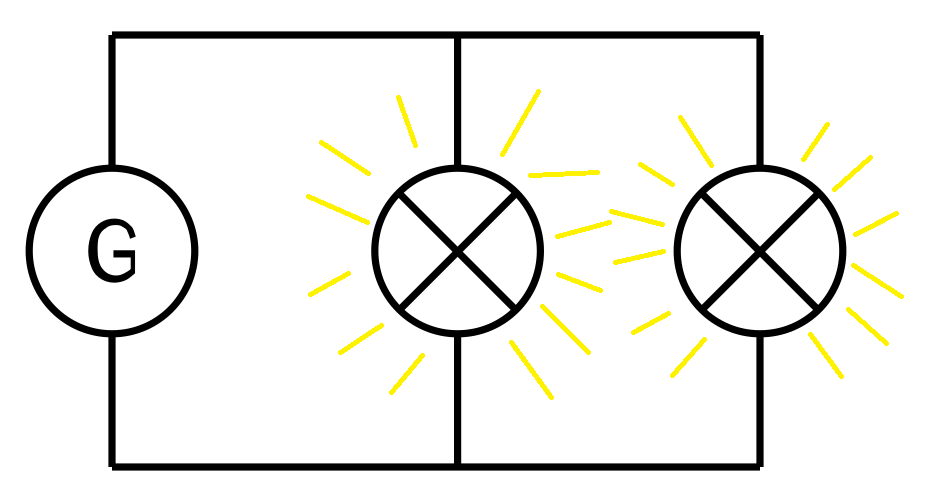
\includegraphics[width=5cm]{images/1d.png}\newline Les lampes brillent avec la même intensité.
\tabularnewline
\hline
2. On dévisse une des lampes 
    & 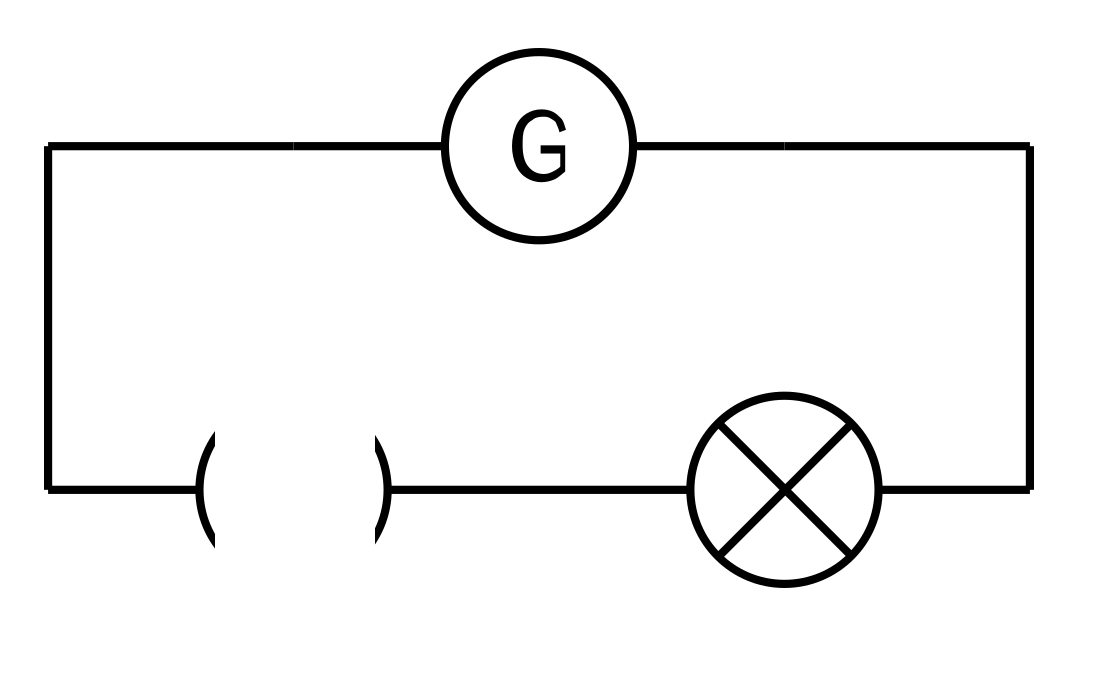
\includegraphics[width=5cm]{images/2s.png}\newline L'autre lampe s'éteint aussi.
    & 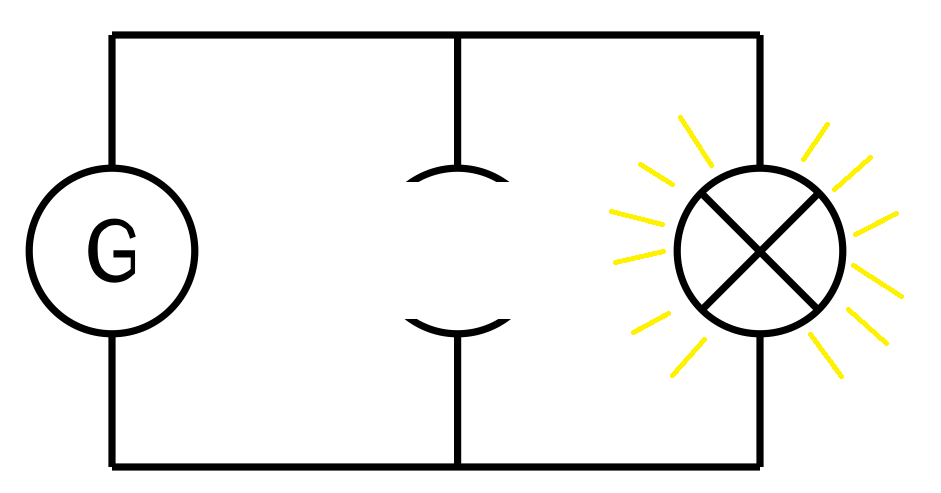
\includegraphics[width=5cm]{images/2d.png}\newline L'autre lampe reste allumée.
\tabularnewline
\hline
3. On échange les lampes de place 
    & Rien ne change. 
    & Rien ne change.
\tabularnewline
\hline
4. On branche un fil électrique aux bornes d'une des lampes
    & 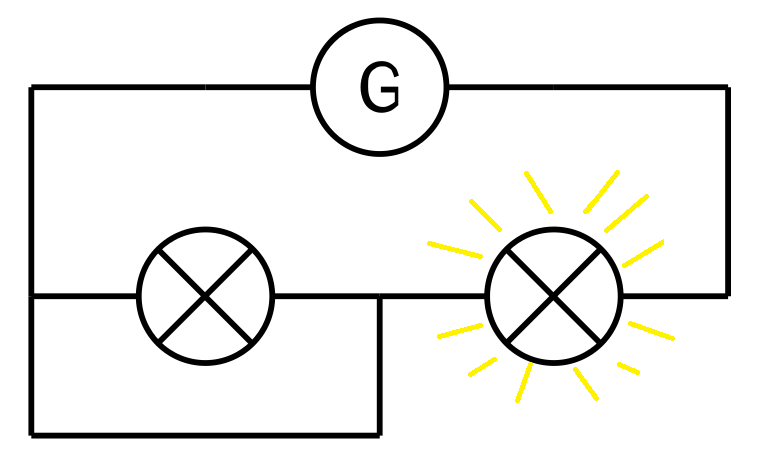
\includegraphics[width=5cm]{images/4s.png}\newline La lampe s'éteint, l'autre brille plus fort.
    & 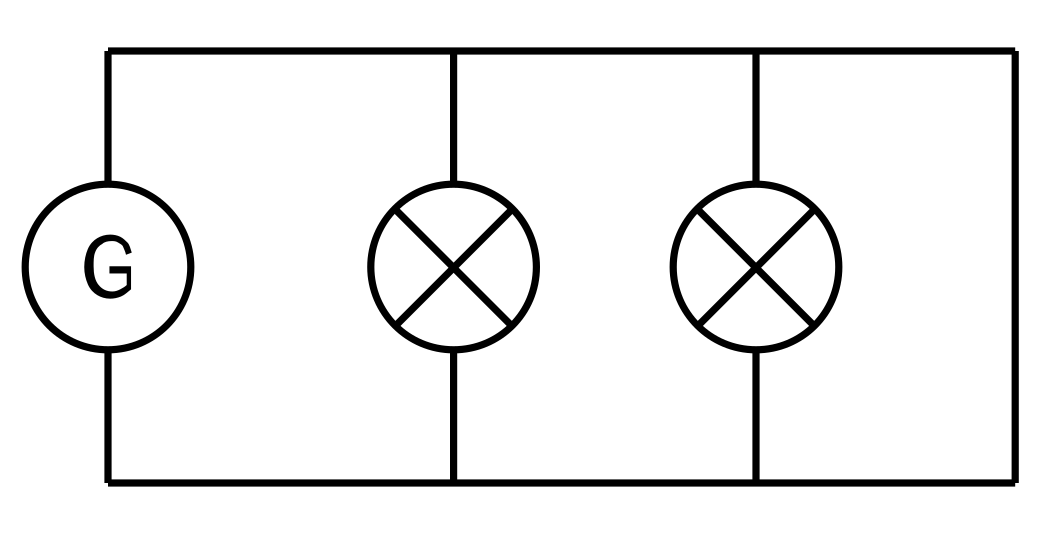
\includegraphics[width=5cm]{images/4d.png}\newline Toutes les lampes s'éteignent.
\tabularnewline
\hline
\end{tabular}

\end{document}